
\documentclass[10pt,a4paper]{article}

%%%%%%%%%%%%%%%%%%%%%%%%%%%%%%%%%%%%%%%%%%%%%%%%%%%%%%%%
%
% Packages and Theorem Environments

\usepackage{graphicx}
\usepackage{psfrag}
\usepackage{epsf}
\usepackage{amsmath,amsfonts,amssymb,latexsym}
\usepackage{enumitem}
\usepackage{algorithmic}
\usepackage{algorithm}
\usepackage[width=160mm,height=240mm,left=35mm,foot=10mm]{geometry}
\usepackage{xcolor}
\usepackage{url}
\usepackage{hyperref}
\usepackage{tikz}



\renewcommand{\theequation}{\thesection.\arabic{equation}}
\newcommand{\makeTiny}[1]{{\tiny #1}}
\newcommand{\work}{\tiny}
\newcommand{\ignore}[1]{}
\newcommand{\startClaims}{\setcounter{claim}{0}}
\newtheorem{theorem}{Theorem}[section]
\newtheorem{corollary}[theorem]{Corollary}
\newtheorem{lemma}[theorem]{Lemma}
\newtheorem{proposition}[theorem]{Proposition}
\newtheorem{conjecture}[theorem]{Conjecture}
\newtheorem{problem}[theorem]{Problem}
\newtheorem{question}[theorem]{Question}
\newtheorem{definition}[theorem]{Definition}
\newtheorem{task}[theorem]{Task}
\newtheorem{claim}{Claim}
\newtheorem{remark}[theorem]{Remark}
\newtheorem{observation}[theorem]{Observation}





\title{MATH 351--004 -- Assignment \#$n$\\
}

\author{Alex Iacob\\
ai9388}

\date{Month XX, XXXX}


%%%%%%%%%%%%%%%%%%%%%%%%%%%%%%%%%%%%%%%%%%%%%%%%%%%%%%%%
%
% Author's definitions


\newcommand{\NN}{\mathbb N}
\newcommand{\ZZ}{\mathbb Z}
\newcommand{\QQ}{\mathbb Q}
\newcommand{\RR}{\mathbb R}

\newcommand{\BB}{\mathcal B}
\newcommand{\ZT}{\mathcal Z}

\newcommand{\Cl}{\operatorname{Cl}}
\newcommand{\Bd}{\operatorname{Bd}}
\newcommand{\row}{\operatorname{row}}
\newcommand{\col}{\operatorname{col}}
\newcommand{\Span}{\operatorname{span}}
\newcommand{\convhull}{\operatorname{conv.hull}}
\newcommand{\tr}{\operatorname{tr}}

\newcommand{\diam}{\operatorname{diam}}

\begin{document}

\maketitle

\begin{center}
{\bf \large Part 2}
\end{center}

\subsection*{Problem 1}

Your solution.

\subsection*{Problem 2}

Your solution.

\subsection*{Problem 3}

Your solution.

\subsection*{Problem 4}

Your solution.


%%%%%%%%%%%%%%%%%%%%%%%%%%%%%%%%%%%%%%%%%%
%Here are some instructions and tips.
%Delete them before handing in your assignment!!!!
%%%%%%%%%%%%%%%%%%%%%%%%%%%%%%%%%%%%%%%%%%

\section*{Appendix: Using \LaTeX}

Thank you for typesetting your solutions in \LaTeX!! This document was created using the ``HW-Template.tex'' source file in the \LaTeX\ folder on MyCourses. The source file  has all of the front matter you should need to get started typesetting your assignment solutions in \LaTeX. To write your solutions, make sure you change the ``title'' and ``author'' fields to your correct information. Then all you need to do is replace ``Your solution'' with your solution. Feel free to play with the formatting if you would like to present your solutions differently.

There are lots of resources for learning \LaTeX\ available online. Usually a google search for whatever problem you are having will lead you to the answer. I don't have any tips for learning \LaTeX\ other than to simply dive in, and learn as you go. This template document should remove most of the confusing aspects of creating a new document, and leave you to work out the best way to write the mathematics.

\subsection*{Handy Resources}

\begin{enumerate}
\item \LaTeX\ is freely available. You can find instructions for installing a \TeX\ distribution here:\\
\url{https://www.latex-project.org/get/}\\
There are also online solutions available, but I would encourage you to work locally. There are a myriad of options for editors, any program that lets you write and edit text will do.
\item There are lots of introductions that will help you get started with \LaTeX\ floating around. I like this one from A.J. Hildebrand:\\
\url{https://faculty.math.illinois.edu/~hildebr/tex/latex-start.html}\\
There is also a WikiBook that you may find useful:\\
\url{https://en.wikibooks.org/wiki/LaTeX}
\item The \TeX\ network on StackExchange is a go-to for quick fixes and answers:\\
\url{https://tex.stackexchange.com/}
\item A short list of symbols and the code for generating them is good to keep at hand. There are lots out there for you to google. I like this one:\\
\url{https://www.caam.rice.edu/~heinken/latex/symbols.pdf}
\item For getting started with TikZ, you can play with the diagrams I have inserted below. Here is a very basic introduction that includes graph-like pictures (from the above linked WikiBook):\\
\url{https://en.wikibooks.org/wiki/LaTeX/PGF/TikZ}\\
If you want all of the gory details, you can find them here:\\
\url{https://texample.net/media/pgf/builds/pgfmanualCVS2012-11-04.pdf}
\end{enumerate}

\subsection*{}

You can insert mathematics inline by wrapping your code in \$ symbols. You should do this whenever referring to names of mathematical objects. For instance, if $G$ is a graph, then you should refer to $G$ as ``$G$'', instead of as ``G''. If you want to write a more complicated string of math symbols, you should use a math environment, like so,
%
\[
\sum_{v\in V(G)}\deg(v)=2|E(G)|.
\]
%
Sums will look better on their own line, rather than inline, as will any expressions that involve symbols under symbols, or symbol over symbols, as will any expression that is ``longish''. As a general rule, if you have more than one relation symbol in your expression (e.g., $=$, $\leq$, $\subset$, etc), it should be in its own math environment.

Unfortunately, putting pictures into \LaTeX\ documents isn't straight forward. If you want to include a diagram as part of your solution, your options are to hand-write a diagram, upload a picture, and include that picture in your tex file (you can find code for inserting figures into tex documents online). This is quick and easy, but has the downside of not looking very nice, and producing large files. Another option is to use your favourite computer program to draw a picture, then insert that picture into your tex file. This will look nicer, and produce a more reasonable-sized file. The fanciest way to produce a diagram is to code one in TikZ. TikZ has lots of great features that will help you draw all sorts of diagrams. But it will require additional effort to learn. I have included a picture (Figure \ref{Kyoto}), and some TikZ diagrams (Figures \ref{GraphG}, \ref{FunStuff}, and \ref{ClebschGraph}) from various presentations of mine to give you some code to play with.

Good luck! And remember to delete this appendix from your solutions!

\begin{figure}[h]
\centering
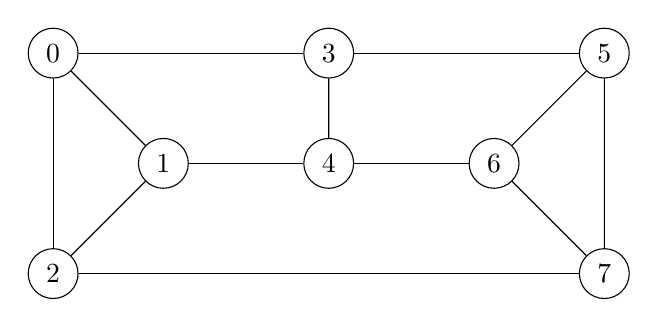
\begin{tikzpicture}[scale=0.7,every node/.style={circle,draw,inner sep=0pt,minimum width=18pt}]
%
\node (0) at (-2,2) {0};
\node (1) at (0,0) {1};
\node (2) at (-2,-2) {2};
\node (3) at (3,2) {3};
\node (4) at (3,0) {4};
\node (5) at (8,2)  {5};
\node (6) at (6,0)  {6};
\node (7) at (8,-2)  {7};
%
\draw (0) edge (1);
\draw (1) edge (2);
\draw (0) edge (2);
\draw (5) edge (6);
\draw (5) edge (7);
\draw (6) edge (7);
\draw (1) edge (4);
\draw (4) edge (6);
\draw (7) edge (2);
\draw (3) edge (4);
\draw (3) edge (5);
\draw (0) edge (3);
%
\end{tikzpicture}
%
\caption{A graph $G$.}\label{GraphG}
\end{figure}

\begin{figure}[h]
\centering
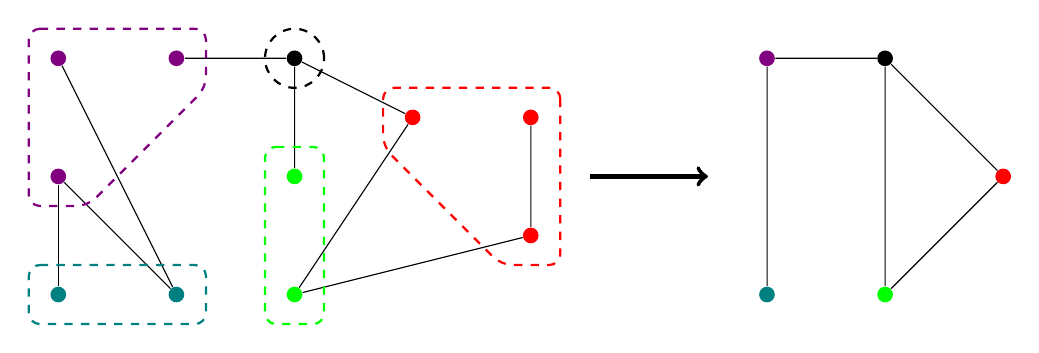
\begin{tikzpicture}[scale=1.5]
\node (1) at (0,1) [circle,inner sep=2pt,fill,violet] {};
\node (2) at (0,0) [circle,inner sep=2pt,fill,violet] {};
\node (3) at (0,-1) [circle,inner sep=2pt,fill,teal] {};
\node (4) at (1,1) [circle,inner sep=2pt,fill,violet] {};
\node (5) at (1,-1) [circle,inner sep=2pt,fill,teal] {};
\node (6) at (2,1) [circle,inner sep=2pt,fill] {};
\node (7) at (2,0) [circle,inner sep=2pt,fill,green] {};
\node (8) at (2,-1) [circle,inner sep=2pt,fill,green] {};
\node (9) at (3,0.5) [circle,inner sep=2pt,fill,red] {};
\node (10) at (4,0.5) [circle,inner sep=2pt,fill,red] {};
\node (11) at (4,-0.5) [circle,inner sep=2pt,fill,red] {};
%
\draw (1) edge (5);
\draw (2) edge (3);
\draw (2) edge (5);
\draw (4) edge (6);
\draw (6) edge (7);
\draw (6) edge (9);
\draw (8) edge (9);
\draw (8) edge (11);
\draw (10) edge (11);
%%
\draw [ultra thick,->] (4.5,0) -- (5.5,0);
%%
\node (a) at (6,1) [circle,inner sep=2pt,fill,violet] {};
\node (b) at (6,-1) [circle,inner sep=2pt,fill,teal] {};
\node (c) at (7,1) [circle,inner sep=2pt,fill] {};
\node (d) at (7,-1) [circle,inner sep=2pt,fill,green] {};
\node (e) at (8,0) [circle,inner sep=2pt,fill,red] {};
%
\draw (a) edge (b);
\draw (a) edge (c);
\draw (c) edge (d);
\draw (c) edge (e);
\draw (d) edge (e);
%%
\draw [rounded corners, thick, dashed,violet] (-0.25,1.25) -- (1.25,1.25) -- (1.25,0.75) -- (0.25,-0.25) -- (-0.25,-0.25) -- cycle;
\draw [rounded corners, thick, dashed,red] (4.25,0.75) -- (4.25,-0.75) -- (3.75,-0.75) -- (2.75,0.25) -- (2.75,0.75) -- cycle;
\draw [rounded corners, thick, dashed,green] (1.75,0.25) -- (2.25,0.25) -- (2.25,-1.25) -- (1.75,-1.25) -- cycle;
\draw [rounded corners, thick, dashed,teal] (-0.25,-0.75) -- (1.25,-0.75) -- (1.25,-1.25) -- (-0.25,-1.25) -- cycle;
\draw [thick,dashed] (2,1) circle [radius=0.25];
\end{tikzpicture}
\caption{Here's some fun stuff!}\label{FunStuff}
\end{figure}

\begin{figure}
\centering
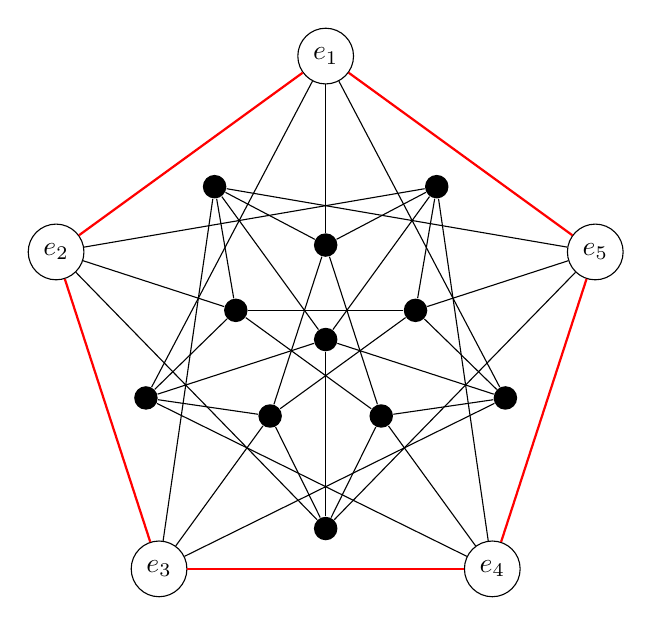
\begin{tikzpicture}[scale=1.2]
%
\node (o1) at (90:3) [circle,draw] {$e_1$};
\node (o2) at (162:3) [circle,draw] {$e_2$};
\node (o3) at (234:3) [circle,draw] {$e_3$};
\node (o4) at (306:3) [circle,draw] {$e_4$};
\node (o5) at (18:3) [circle,draw] {$e_5$};
%
\node (m1) at (270:2) [circle,inner sep=3pt,fill] {};
\node (m2) at (342:2) [circle,inner sep=3pt,fill] {};
\node (m3) at (54:2) [circle,inner sep=3pt,fill] {};
\node (m4) at (126:2) [circle,inner sep=3pt,fill] {};
\node (m5) at (198:2) [circle,inner sep=3pt,fill] {};
%
\node (i1) at (90:1) [circle,inner sep=3pt,fill] {};
\node (i2) at (162:1) [circle,inner sep=3pt,fill] {};
\node (i3) at (234:1) [circle,inner sep=3pt,fill] {};
\node (i4) at (306:1) [circle,inner sep=3pt,fill] {};
\node (i5) at (18:1) [circle,inner sep=3pt,fill] {};
%
\node (c) at (0:0) [circle,inner sep=3pt,fill] {};
%%
\draw (o1) edge[thick,red] (o2);
\draw (o2) edge[thick,red] (o3);
\draw (o3) edge[thick,red] (o4);
\draw (o4) edge[thick,red] (o5);
\draw (o5) edge[thick,red] (o1);
%
\draw (i1) edge (i3);
\draw (i3) edge (i5);
\draw (i5) edge (i2);
\draw (i2) edge (i4);
\draw (i4) edge (i1);
%
\draw (c) edge (m2);
\draw (c) edge (m3);
\draw (c) edge (m4);
\draw (c) edge (m5);
\draw (c) edge (m1);
%
\draw (i1) edge (m4);
\draw (m4) edge (i2);
\draw (i2) edge (m5);
\draw (m5) edge (i3);
\draw (i3) edge (m1);
\draw (m1) edge (i4);
\draw (i4) edge (m2);
\draw (m2) edge (i5);
\draw (i5) edge (m3);
\draw (m3) edge (i1);
%
\draw (o1) edge (i1);
\draw (o2) edge (i2);
\draw (o3) edge (i3);
\draw (o4) edge (i4);
\draw (o5) edge (i5);
%
\draw (o1) edge (m2);
\draw (o1) edge (m5);
%
\draw (o2) edge (m3);
\draw (o2) edge (m1);
%
\draw (o3) edge (m4);
\draw (o3) edge (m2);
%
\draw (o4) edge (m3);
\draw (o4) edge (m5);
%
\draw (o5) edge (m4);
\draw (o5) edge (m1);
\end{tikzpicture}
\caption{A drawing of the \href{https://en.wikipedia.org/wiki/Clebsch_graph}{Clebsch Graph}.}\label{ClebschGraph}
\end{figure}

\begin{figure}
\centering
\includegraphics[scale=0.28]{JCCA2016.jpg}
\caption{A photo containing several famous combinatorialists as well as the professor for this course. Can you find me?}\label{Kyoto}
\end{figure}


\end{document} 




















